\section{Impact of nuclear PDFs}
\label{app:npdf}

The predictions presented in this work neglect nuclear effects in the tungsten target of the detector, which we model as an isospin combination of free protons and neutrons.
%
In this appendix we quantify the impact of nPDF uncertainties~\cite{Klasen:2023uqj,Ethier:2020way} on DIS differential distributions in the fiducial region of Eq.~(\ref{eq:fiducial}).
%
For this purpose, we evaluate \yadism NLO structure functions in the ZM-VFNS scheme with target-mass corrections for three nPDF sets, namely nNNPDF3.0~\cite{AbdulKhalek:2022fyi}, EPPS21~\cite{Eskola:2021nhw} and nCTEQ15HQ~\cite{Kovarik:2015cma,Duwentaster:2022kpv}, in all cases at NLO accuracy, and compare with the corresponding free-nucleon baseline. 
%
See also~\cite{Francener:2025tyh} for a related study.

Fig.~\ref{fig:npdf} shows differential distributions in $x_{\rm Bj}$, $Q^2$ and $y$ for muon and neutrino DIS on a tungsten target at the reference energy of $E_\ell=1$~TeV  in the fiducial region of the benchmark for these three nPDF sets as well as for NNPDF4.0.
%
The bottom panels display the ratio of each prediction to the corresponding free-nucleon case, namely the $A=1$ variants of each nPDF determination.
%
Note that the same nPDF dependence would be found should one use the NLO-matched event generators (following the findings of Sect.~\ref{sec:inclusive}), since the observables considered here do not depend on the modelling of the hadronic final state, and hence showing the \yadism predictions is sufficient. 


%%%%%%%%%%%%%%%%%%%%%%%%%%%%%%%%%
\begin{figure}[!tbp]
  \centering
  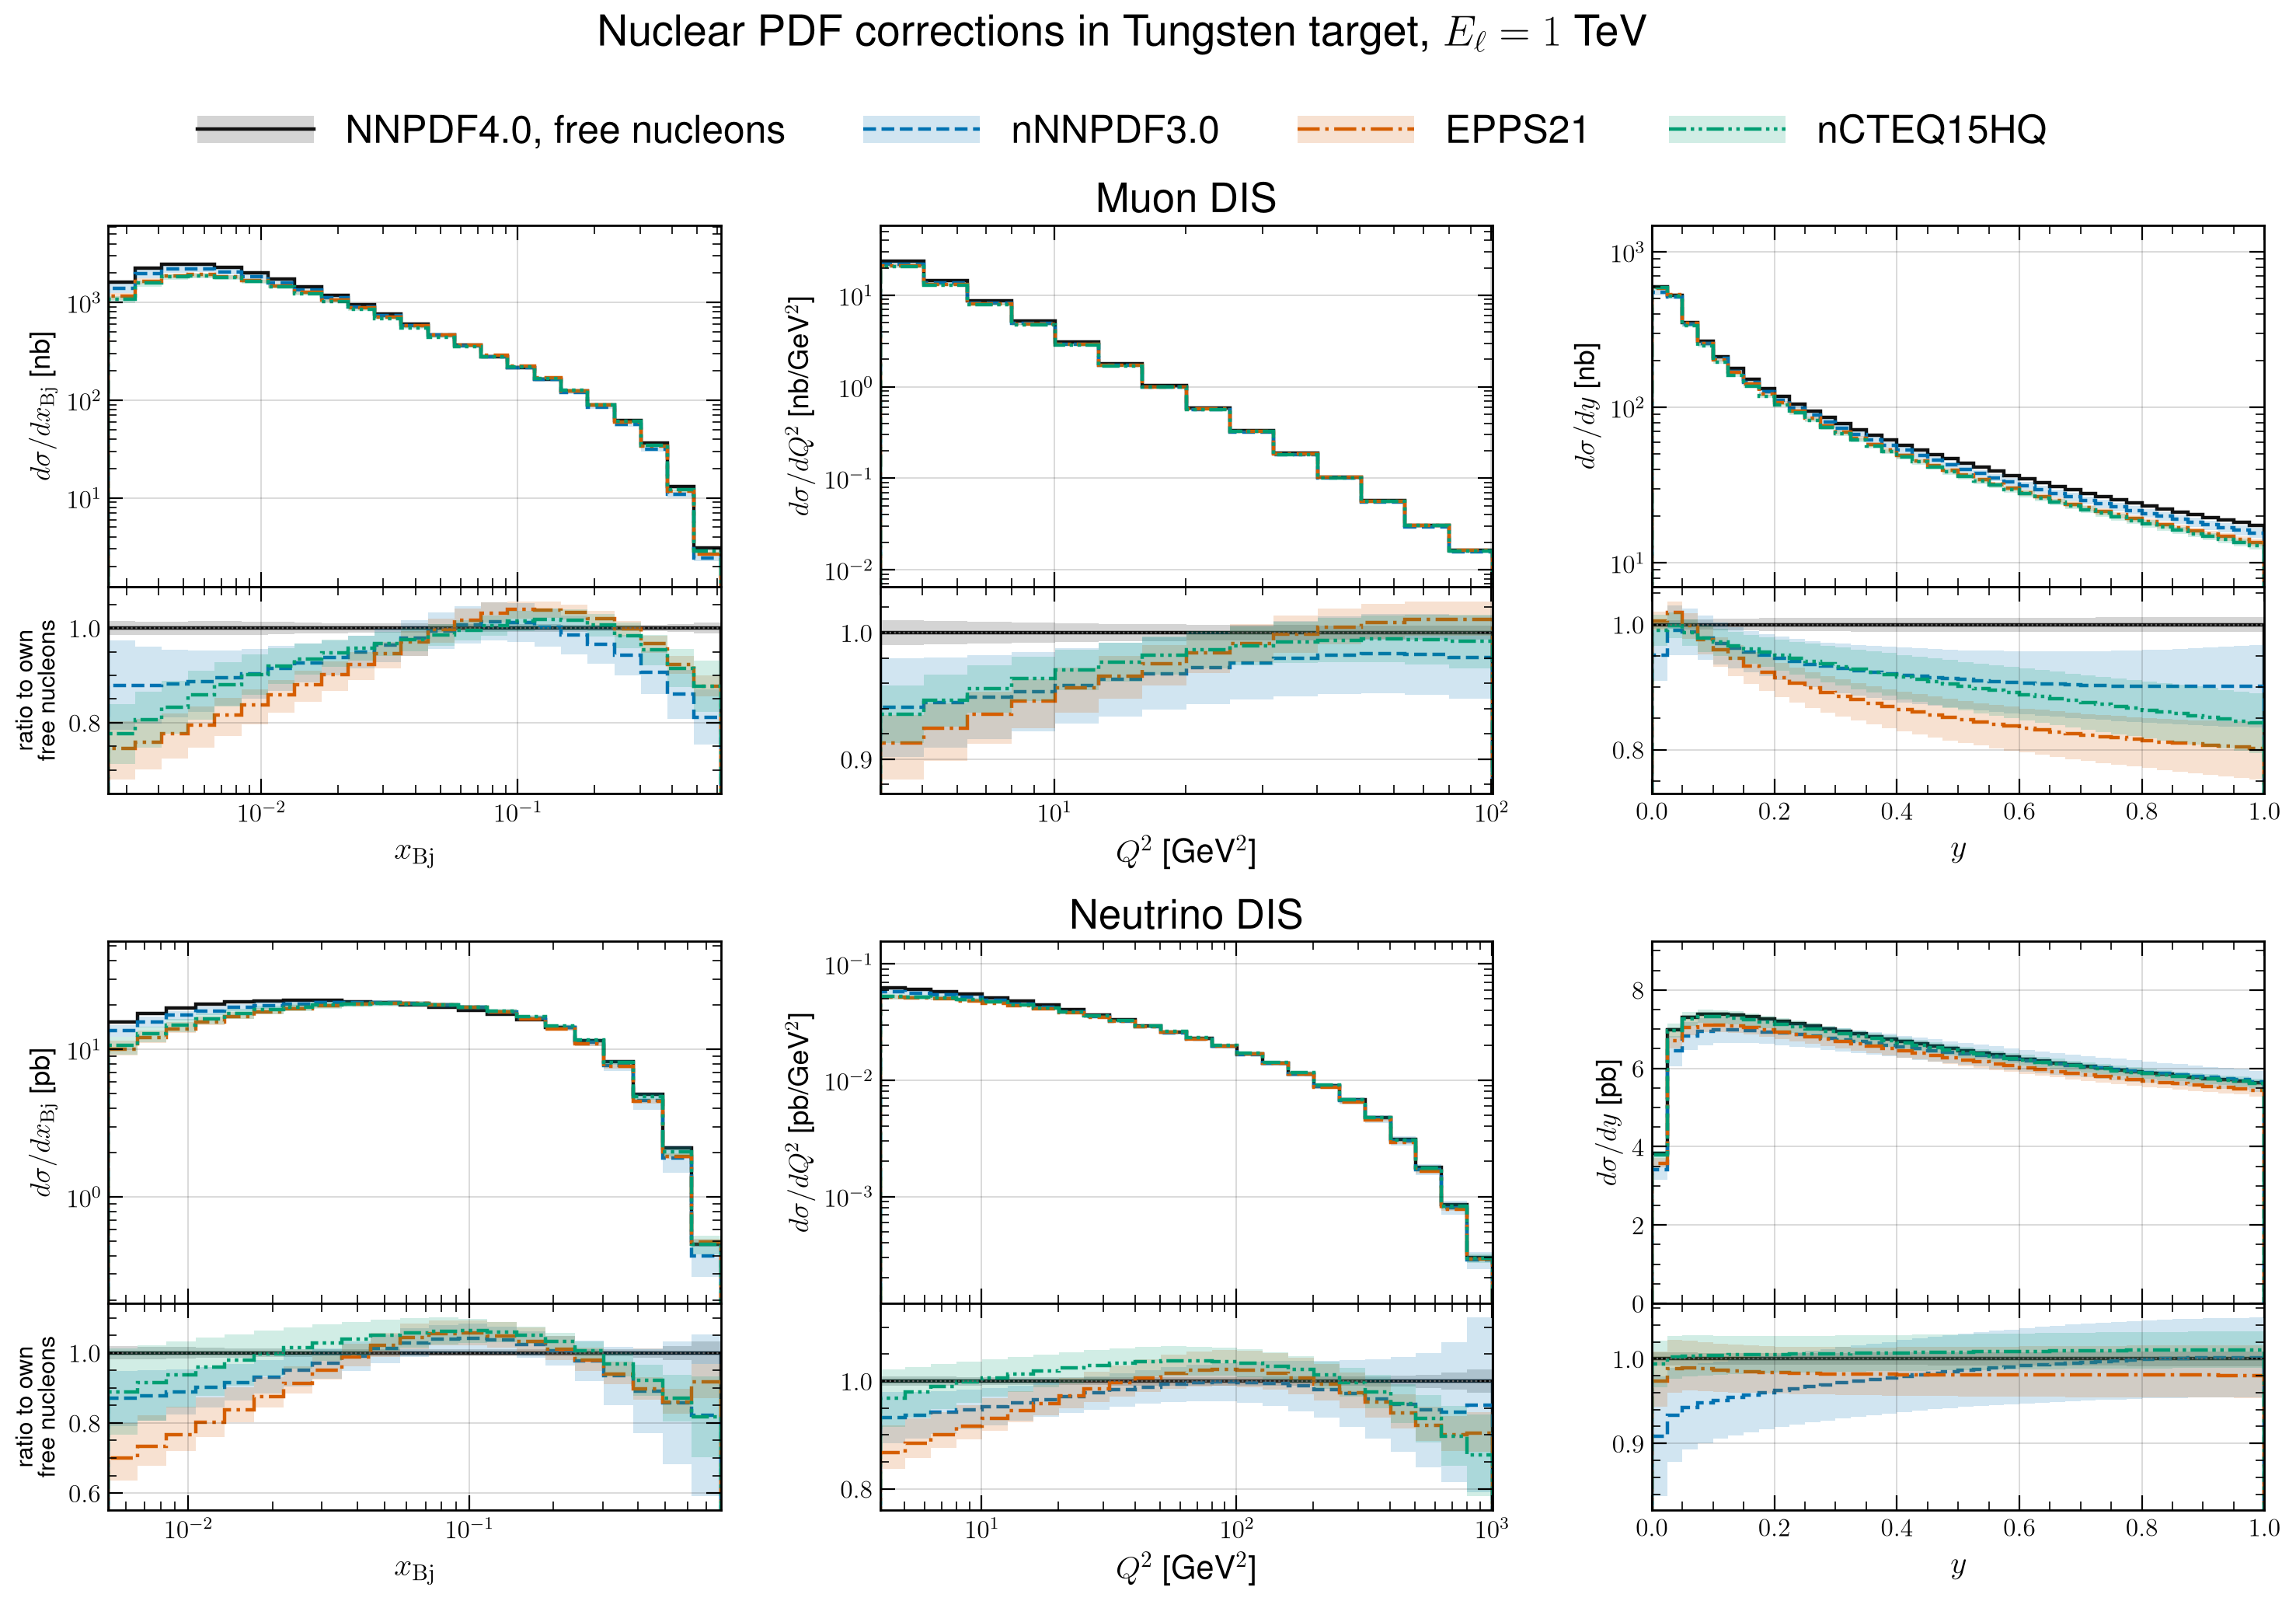
\includegraphics[width=0.99\textwidth]{figures/pp_npdf_impact.png}
  \caption{Differential inclusive distributions in $x_{\rm Bj}$, $Q^2$ and $y$ for muon (top) and neutrino (bottom) DIS on a tungsten target at $E_\ell=1$~TeV  in the fiducial region of Eq.~(\ref{eq:fiducial}), computed with \yadism\ at NLO in the ZM-VFNS and with TMCs.
    %
The baseline predictions, evaluated with NNPDF4.0, are compared with three nPDF sets nNNPDF3.0~\cite{AbdulKhalek:2022fyi}, EPPS21~\cite{Eskola:2021nhw} and nCTEQ15HQ~\cite{Kovarik:2015cma,Duwentaster:2022kpv}. 
%
The bottom panels display the ratio of each prediction to the corresponding free-nucleon case, namely the $A=1$ variants of each nPDF determination.}
  \label{fig:npdf}
\end{figure}
%%%%%%%%%%%%%%%%%%%%%%%%%%%%%%

From Fig.~\ref{fig:npdf} one observes that nPDF effects are in general sizeable, though the associated uncertainties remain large.
%
Indeed, nPDF uncertainties are $2$ to $6$ times larger than the free-nucleon one.
%
In general, predictions from the three different nPDF sets are in qualitative agreement, mostly overlapping between their $1\sigma$ uncertainties.
%
nPDF-associated shifts tend to be smaller for neutrino DIS (where a nuclear ratio of unity is still allowed within uncertainties, except at small $x$ and low $Q^2$) than for muon DIS, where a non-unity value of the nuclear ratio is clearly preferred.
%
The latter is especially true for the $y$ distribution, the low-$Q^2$ region, and the large-$x$ (EMC effect) and small-$x$ (shadowing) regions.

All in all, Fig.~\ref{fig:npdf} indicates that nPDF corrections must be accounted for when producing predictions for FASER observables and related simulations, since they are comparable to the NNLO corrections for muon DIS and larger than the spread between NLO-matched generators for both NC and CC scattering.
%
Furthermore, this comparison confirms that FASER data itself should provide excellent opportunities to constrain nuclear PDFs alongside the free-nucleon ones, as already demonstrated in~\cite{Cruz-Martinez:2023sdv}.
%
Using the pipeline presented in this work, NLO-matched predictions for the various generators considered accounting for nPDF effects are straightforward and can be implemented directly at the run card level.
%
In the specific case of \powheg, its reweighting functionality implies that no additional generation campaign is required.



